%!TEX root = ../dokumentation.tex
\chapter{Kubernetes}

Um die in der Vorlesung behandelte Orchestrierung der Docker-Container zu behandeln, wurde ein Kubernetes Cluster auf Azure erstellt.

\section{Konvertierung Docker Compose zu Kubernetes}

Um die Docker-Compose Umgebung in Kubernetes umsetzen zu können, wurde zunächst die docker-compose.yml konvertiert.

Hierzu wurde das Kubernetes Tool Kompose verwendet.

\begin{verbatim}
	$ kompose convert -o k8s.yml
\end{verbatim}

Anschließend wurde die Kubernetes Deployment Datei auf einen bei Azure zugewiesenen Dateispeicher hochgeladen. In der Azure Cloud-Console konnte somit initial der Cluster initialisiert werden.

\begin{figure}[h!]
 \centering
 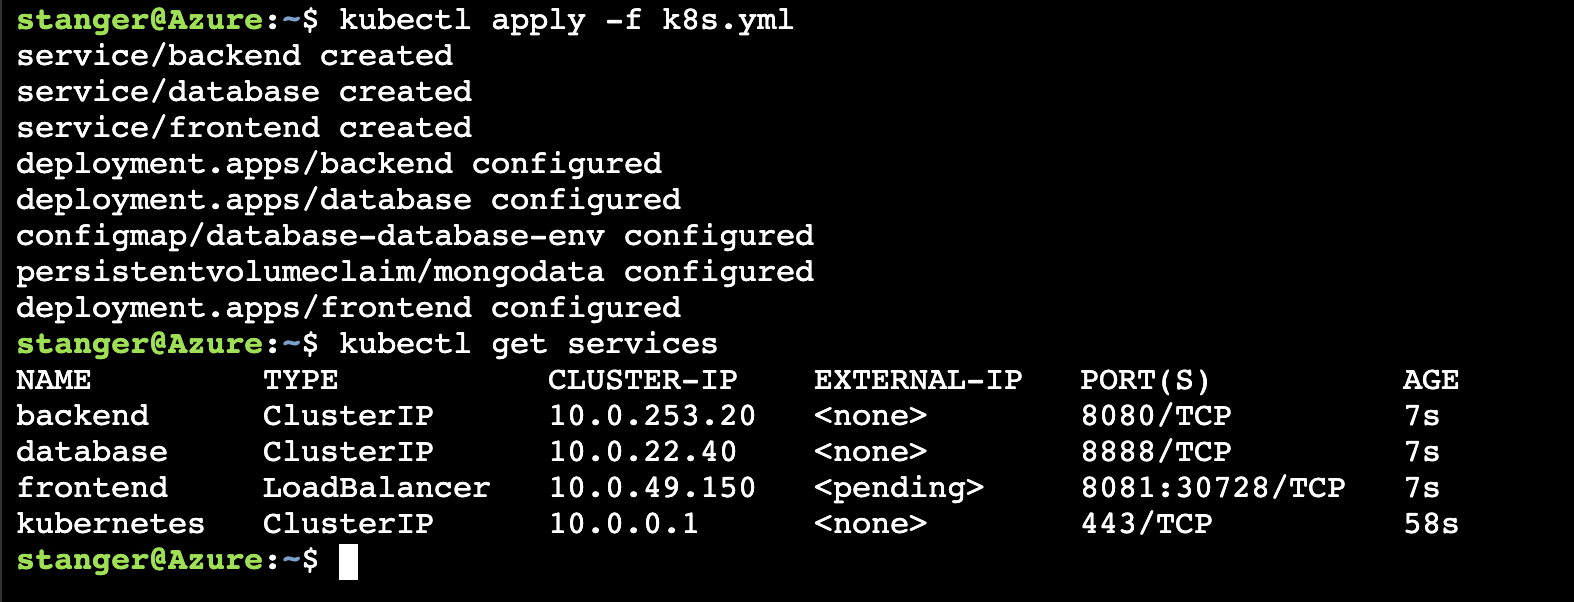
\includegraphics[width=150mm]{images/azure.png}
 \caption{Azure Service Deployment}
 \label{fig:azure-deployment}
\end{figure}

\section{Probleme bei der Verwendung von Kubernetes}
Nach dem Deployment des Kubernetes Clusters war die Website zwar unter der dem LoadBalancer zugeteilten IP-Adresse erreichbar, jedoch war keine Kommunikation zwischen Frontend und Backend Pod möglich. Hierfür wurden verschiedenste Lösungsansätze umgesetzt, wobei jedoch keiner dieser Ansätze das Problem gelöst hat. 

Ein Auszug aus dem Log des Frontend-Pods zeigt dieses Problem auf.

\begin{figure}[h!]
 \centering
 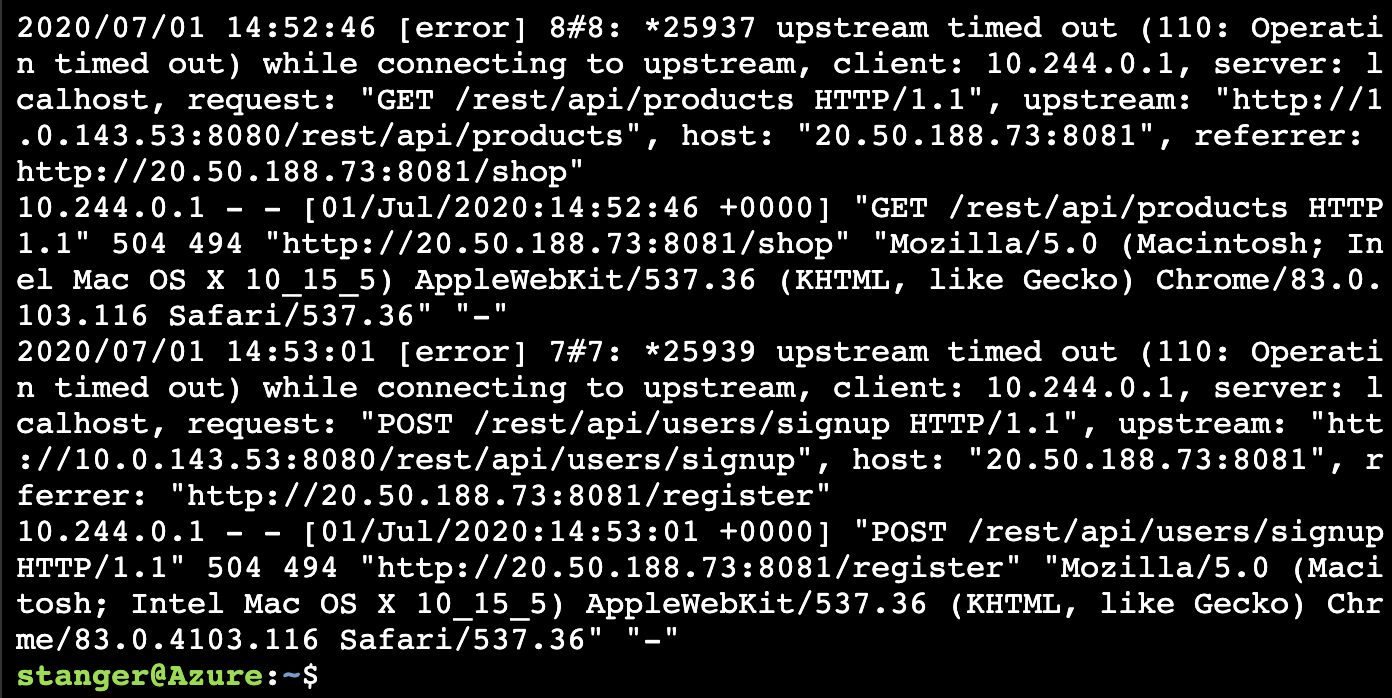
\includegraphics[width=150mm]{images/kubernetes-failure.png}
 \caption{Kubernetes Communication Failure}
 \label{fig:kubernetes-failure}
\end{figure}

Hierbei ist deutlich zu erkennen, dass das Backend mit einer IP-Adresse aufgelöst wird, die nicht im Cluster vorhanden ist. Dieses Problem konnte im weiteren Prozess leider nicht behoben werden, weshalb die volle Funktionalität unter Kubernetes nicht weiter entwickelt werden konnte.